\documentclass[a4j,12pt]{jarticle}
%\setlength{\topmargin}{-25mm}
\usepackage[dvipdfmx]{graphicx}
\usepackage{here}
\usepackage{theorem}
\usepackage{amsmath}
\usepackage{amsfonts}
\usepackage{ascmac}
\usepackage{bm}
\usepackage{comment}
%\usepackage{listings,jlisting}
\usepackage{listings}
\usepackage{url}
\usepackage{wrapfig}
\usepackage{cite}
\usepackage[round]{natbib}
\usepackage[top=30truemm,bottom=30truemm,left=25truemm,right=25truemm]{geometry}

\newtheorem{theo}{定理}[section]
\newtheorem{defi}{定義}[section]
\newtheorem{lemm}{命題}[section]

\title{混合射影正規分布によるクラスタリングについて}   %タイトル
\author{小坪琢人}   %著者
\date{\today}   %日付

\makeatletter
\def\theequation{\thesection.\arabic{equation}}   %数式番号を(章.式)形式
\@addtoreset{equation}{section}
\def\thefigure{\thesection.\arabic{figure}}   %図番号を(章.図)形式
\@addtoreset{figure}{section}
\def\thetable{\thesection.\arabic{table}}   %表番号を(章.表)形式
\@addtoreset{table}{section}
\def\tr{\mathop{\operator@font tr}\nolimits}
\def\grad{\mathop{\operator@font grad}\nolimits}
\def\St{\mathop{\operator@font St}\nolimits}
\def\Hess{\mathop{\operator@font Hess}\nolimits}
\def\D{\mathop{\operator@font D}\nolimits}
\def\sym{\mathop{\operator@font sym}\nolimits}
\makeatother

\setlength\textfloatsep{1pt}
\setlength\floatsep{1pt}

\begin{document}
%\bibliographystyle{jecon} % 経済学などでよく使われる
\bibliographystyle{plainnat}

%%%%%%%%%%% タイトルはいらない %%%%%%%%%%%%%%%%%%%
%\maketitle   %タイトルを付ける
\setlength{\baselineskip}{20pt}   %行間幅
\pagenumbering{roman}   %目次ページ番号のスタイル
\tableofcontents   %目次を付ける
\listoffigures   %図目次を付ける
\listoftables   %表目次を付ける
\clearpage   %目次と本文を分ける
\pagenumbering{arabic}   %本文ページ番号のスタイル

%%%%%これ以下, 本文%%%%%

\section{はじめに}
%%% 2-3ページ  %%%%

円周上や球面上のデータを扱う統計手法を方向統計学といい, 近年多様体上の統計分析手法として, 注目を集めている. 方向統計学とは風向データ, 渡り鳥の移動方向データなどの角度観測値を含むデータを対称とする統計学である. 単位超球面上 $(\mathbb{S}^{p-1})$ に分布するようなデータをユークリッド空間上のデータとして扱い, ベクトル間の類似度の指標にユークリッド距離を用いると良い解析が行えない場合がある. そこで, データを多様体上の確率分布として扱うことで, 超球面上でのベクトル間の類似度指標を用いることができ, 加えて数学的モデルを作る際に低次元で考えられるなどの利点がある. 円周あるいは超球面上の分布を生成するいくつかの方法が知られている. 代表的なものとして, 巻き込み法, 射影法, 条件付法, 投影法である. 本研究では射影法を用いた射影分布によるクラスタリングについて議論する.

代表的なクラスタリング手法として, $k$平均法が挙げられる. $k$平均法は, 各データと各クラスタの中心のユークリッド距離を最小化することで, 各データをクラスタリングする. しかし確率変数が円周上や球面上に値をとるようなデータに対して, ユークリッド空間のクラスタリングを前提とした$k$平均法はしばしば誤った分類結果をもたらすことがある. \citet{SKMcluster}は, ユークリッド距離に基づく非類似度の尺度を単位球面上に射影したコサイン非類似度の最小化に基づく超球面上の$k$平均法を提案した. この手法ではデータの単位方向ベクトルと各クラスタにおける重心ベクトルとのコサイン非類似度を最小化することで, 各データをクラスタリングする. 

超球面上の$k$平均法は確率モデルを仮定しないノンパラメトリックな手法であるのに対し,  パラメトリックな超球面上のクラスタリング手法として, \citet{Gopal}による von Mises Fisher 分布の混合分布を用いた手法がある. 単位超球面上の分布として知られる, von Mises Fisher 分布を用いて, MCMCサンプリングにより高次元データのクラスタリングを行う. MCMCを用いることで求める事後分布のパラメータの平均値, 標準偏差を求めることができ, さらに事後分布を利用したモデルの妥当性の検証を行うことができる. 本研究では方向データの分布として知られる, 射影正規分布の混合分布によるクラスタリングの性能評価を行う. 混合分布のコンポーネント数の評価指標には\citet{WAIC}によるWAIC基準を用いる. クラスターごとの特徴量を確認することで, 混合射影正規分布によるクラスタリングの妥当性を検証する.

%%%%%%%%%%%%%%%%%%%%%%%%%%%%%%%%%%%%%%%%%%%%%%%%%%%%%%%%%%%%%%%%%%%%%%%%%%%%%%%%%%%
%%%%%%%%%%%%%%%%%%%%%%%% senction2 混合分布 %%%%%%%%%%%%%%%%%%%%%

\section{理論}

球面上における平均方向の定義, 射影正規分布の確率密度関数について示し, パラメーターを変化させて射影正規分布の確率分布の概形について示す. クラスタリング分析に用いる, 混合射影正規分布について定義し, MCMCによるパラメーターの推定方法について述べる.  

\subsection{射影正規分布}

射影分布は平面または空間上の放射状の射影によって得られる. 一般的には, 多変量正規ベクトルをノルムで割ることで, 単位超球面上への射影分布が得られる. 多変量正規ベクトル($k$次元)を$X$として, $k \geq 2$ の場合には, 単位超球面上への単位ベクトル $U$ は $U = X/\|X\|$ で表される. このとき$U$は$k$次元の一般化射影正規分布に従い, $U \sim \mathcal{PN}_k(\bm \mu,\Sigma)$と表せる. 一般化射影正規分布は, パラメータ$\bm \mu, \Sigma$をもち, \citet{PML}で, $\Sigma = \mathcal{I}$と定義されていた射影正規分布を一般化したものである. $\mathcal{PN}_k(\bm \mu,\mathcal{I})$は平均方向$\bm \mu$に対して, 単峰性かつ対称の分布となるが, $\mathcal{PN}_k(\bm \mu,\Sigma)$では非対称分布もしくは二峰性分布となる. ここで超球面上における平均方向について, 円周上の例を用いて説明する. $\pi/3$ラジアン(実線)と$5\pi/3$ラジアン(実線)の平均方向について考える. 算術平均では$(\pi/3 + 5\pi/3)/2 = \pi$より, $\pi$ラジアン(破線)となるが, 図\ref{sample_mu1}より$2$つのベクトルの平均方向としては不適切なことが分かる. よって図\ref{sample_mu2}に示したように, これらの角度を円周上の点 $(\cos \frac{\pi}{3},\sin \frac{\pi}{3}) = (\frac{1}{2},\frac{\sqrt{3}}{2}),\ (\cos \frac{5\pi}{3}, \sin \frac{5\pi}{3}) = (\frac{1}{2},- \frac{\sqrt{3}}{2})$ と表し, 円周上における2つの座標の平均を取ると $\frac{1}{2} (\cos 0, \sin 0)$となり, ベクトルの平均方向は$0$ラジアン(破線)となる. 

\begin{figure}[bp]
 \begin{tabular}{c}
 \begin{minipage}{0.5\hsize}
  \begin{center}
   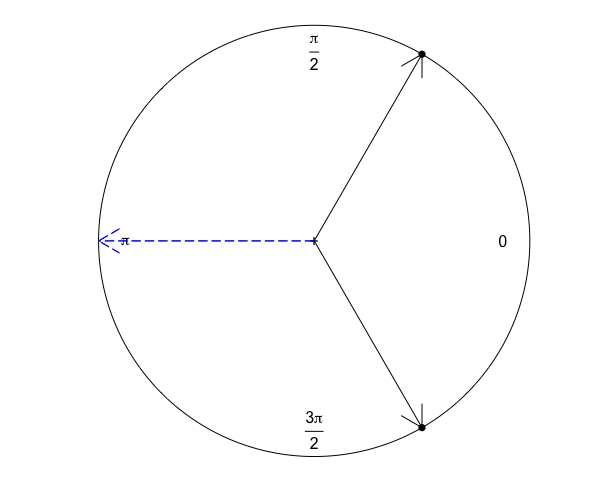
\includegraphics[clip,height= 60mm]{data/sample_False.png}
\caption{算術平均による平均の定義}
\label{sample_mu1}
  \end{center}
 \end{minipage}
 \begin{minipage}{0.5\hsize}
  \begin{center}
 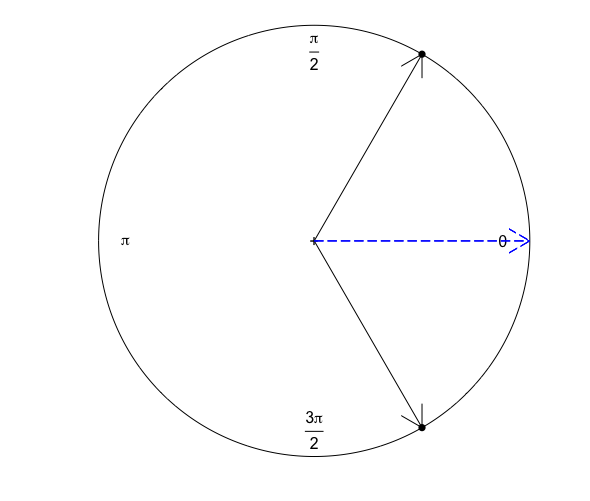
\includegraphics[clip,height= 60mm]{data/sample_True.png}
\caption{円周上における平均方向の定義}
\label{sample_mu2}
  \end{center}
 \end{minipage}
\end{tabular}
\label{sample_mu}
\end{figure}

\newpage
\citet{PN1}によると, $\mathcal{PN}_2(\bm \mu,\Sigma$)の円形データの場合, 単位円上の方向を表す$U = (\cos\Theta, \sin\Theta)^T$における$\theta$の確率密度を式(\ref{PNC})に示す.

\begin{eqnarray}
\label{PNC}
p(\theta; \bm \mu, \Sigma) = \frac{1}{2\pi A(\theta)}|\Sigma|^{-\frac{1}{2}}
\exp(C)\left\{1 + \frac{B(\theta)}{\sqrt{A(\theta)}} \frac{\Phi \left(\frac{B(\theta)}{\sqrt{A(\theta)}}\right)}{\phi \left(\frac{B(\theta)}{\sqrt{A(\theta)}}\right)}\right\} I_{[0,2\pi)}(\theta),
\end{eqnarray}

\noindent
ここで, $\bm u^T = (\cos\theta,\sin\theta), \ A(\theta) = \bm u^T\Sigma^{-1}\bm u, \ B(\theta) = \bm u^T \Sigma^{-1} \bm \mu, \ C = -\frac{1}{2} \bm \mu^T \Sigma^{-1} \bm \mu$であり, $I_{[0,2\pi)} (\cdot)$は指示関数, $\Phi(\cdot), \phi(\cdot)$ は標準正規分布の確率密度関数と累積密度関数である. 指示関数とはある元が, 任意の集合に属する場合$1$を, そうでない場合$0$を示す関数である. 以下に定義式を示す.

\begin{eqnarray*}
I_{[0,2\pi)}(\theta) = \left\{
    \begin{array}{ll}
      1 \quad (0 \leq \theta < 2\pi), \\
      0 \quad \mbox{other}, \\
\end{array}
\right.
\end{eqnarray*}

射影正規分布において対称分布, 非対称分布, 二峰性分布となる例をそれぞれ図\ref{sample_pnc1}, 図\ref{sample_pnc2}, 図\ref{sample_pnc3}に示す. 

\begin{figure}[bp]
\begin{center}
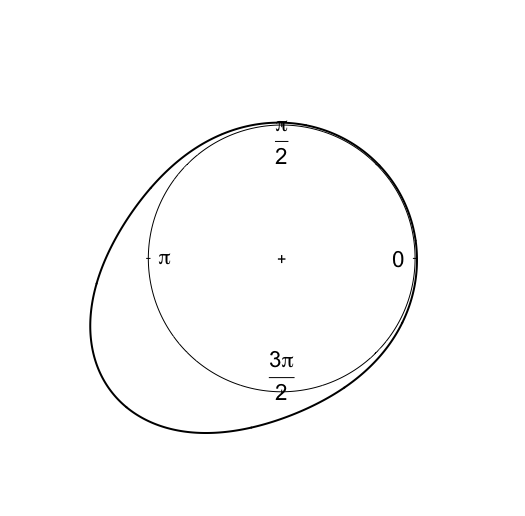
\includegraphics[clip,height= 80mm]{data/sample_symmetry.png}
\caption[対称な射影正規分布]{
$\bm \mu = \begin{pmatrix} -1.2 \\ -0.95 \\ \end{pmatrix}, \ \Sigma = \begin{pmatrix}  1 & 0 \\ 0 & 1 \\ \end{pmatrix}$
とした場合の対称な射影正規分布.}
\label{sample_pnc1}
\end{center}
\end{figure}

\begin{figure}[tbp]  
\begin{center}
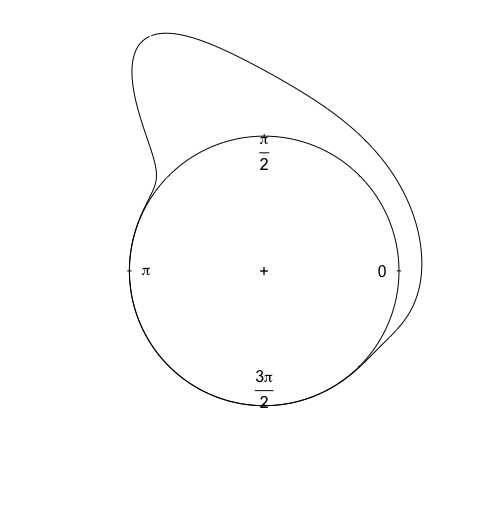
\includegraphics[clip,height= 80mm]{data/sample_asymmetry.png}
\caption[非対称な射影正規分布]{
$\bm \mu = \begin{pmatrix} -0.19 \\ 2.09 \\ \end{pmatrix}, \ \Sigma = \begin{pmatrix} 2.49 & -1.85 \\ -1.85 & 1.96 \\ \end{pmatrix}$ とした場合の非対称な射影正規分布.}
\label{sample_pnc2}
\end{center}
\end{figure}

\begin{figure}[tbp]  
\begin{center}
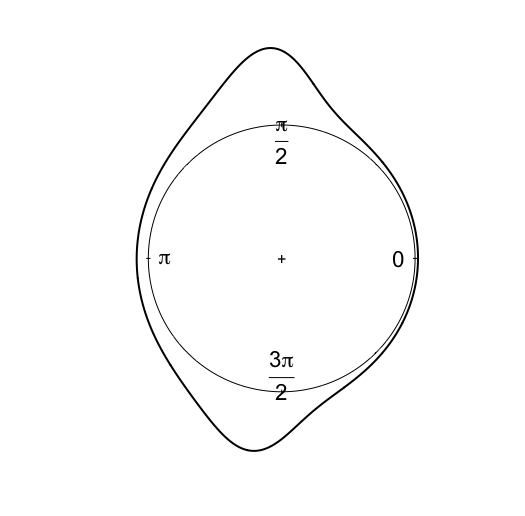
\includegraphics[clip,height= 70mm]{data/sample_bimodal.png}
\caption[二峰性となる射影正規分布]{
$\bm \mu = \begin{pmatrix} -0.24 \\ 0.15 \\ \end{pmatrix}, \ \Sigma = \begin{pmatrix} 0.209 & 0.068\\ 0.068 & 2.25 \\ \end{pmatrix}$ とした場合の二峰性となる射影正規分布.}
\label{sample_pnc3}
\end{center}
\end{figure}

% Wang and Gelfand(2013) によると各パラメータの単一の影響は良く分かっていない. だから各パラメータを細かく説明するのは困難である. しかしこの分布の柔軟な特性は予測などにおいて便利である.

\citet{GPN}によると, $\mathcal{PN}_3(\bm \mu,\Sigma$)の球形データの場合, 単位球面上の方向を表す$U = (\cos\Theta_1 \sin \Theta_2, \sin\Theta_1 \sin \Theta_2, \cos \Theta_2)^T$における$\bm \theta = (\theta_1, \theta_2)^T$の確率密度を式(\ref{PNS})に示す.

%\footnotesize %式を小さくする
\begin{eqnarray}
\label{PNS}
p(\bm \theta; \bm \mu, \Sigma) &=& \left(\frac{1}{2\pi A(\bm \theta)}\right)^{\frac{3}{2}} |\Sigma|^{-\frac{1}{2}}
\exp(C) \nonumber \\ 
&& \hspace{-1.5cm} \times \left( \left[1 + D(\bm \theta) \frac{\Phi \{D(\bm \theta)\}}{\phi \{D(\bm \theta)\}} \right] D(\bm \theta) + \frac{\Phi \{D(\bm \theta)\}}{\phi \{D(\bm \theta)\}} \right) I_{[0,2\pi)}(\theta_1) I_{[0,\pi)}(\theta_2),
\end{eqnarray}
%\normalsize

\noindent
ここで, $\bm u^T = (\cos\theta_1 \sin \theta_2, \sin\theta_1 \sin \theta_2, \cos \theta_2), 
\ D(\bm \theta) = B(\bm \theta) A^{-\frac{1}{2}}(\bm \theta), \ A(\bm \theta) = \bm u^T \Sigma^{-1} \bm u,\\ B(\bm \theta) = \bm u^T \Sigma^{-1} \bm \mu, \ C = -\frac{1}{2} \bm \mu^T \Sigma^{-1} \bm \mu$であり, $I_{[0,2\pi)} (\cdot), I_{[0,\pi)}(\cdot)$は指示関数, $\Phi(\cdot), \phi(\cdot)$ は標準正規分布の確率密度関数と累積密度関数である. 

\subsection{混合射影正規分布}
\if0
%%%%%%%%%%%%%%%%  円周 %%%%%%%%%%%%%%%%%%%%%%%%%%
%%%% 重複するからいらない %%%%%
$m$個のユニットからなる 円周上の射影正規分布の混合分布は以下のように定式化できる. 

\begin{eqnarray*}
\label{MPNC}
p(\theta;\bm w,\bm \mu, \Sigma) = \sum^m_{j=1} w_j \mathcal{PN}_2(\theta;\bm \mu_j, \Sigma_j),
\end{eqnarray*}

\noindent
ただし, $w_j$は混合比率であり, $0 < w_j < 1$, $\sum^m_{j=1} w_j = 1$を満たす. 混合射影正規分布におけるパラメータは, $w, \bm \mu_j, \Sigma_j$であるが, パラメータに識別可能性を保持するという制約を加えると共分散行列 $\Sigma$は

\begin{eqnarray}
\label{SIGMA2}
 \Sigma_j = \left(
    \begin{array}{cc}
      \tau_j^2 & \rho_j \tau_j \\
      \rho_j \tau_j & 1
    \end{array}
  \right),
\end{eqnarray}

\noindent
と定義されるので, パラメータベクトルは$\bm \eta = (w_1, \dots, w_m, \bm \mu_1, \dots, \bm \mu_m, \tau_1, \dots, \tau_m, \rho_1, \dots, \rho_m)^T$, パラメータベクトルの次元は $d = 4m$ となる. 各パラメータの事前分布を $\bm \mu_j \sim N(\bm 0, 10^5 \bm I_2)$, $\tau_j \sim \mathrm{half Cauchy}(0,5)$, $\rho_j \sim U(-1,1)$, $\bm w \sim Dirichlet(2,2, \dots, 2)$ と設定する. ここで混合比率$\bm w$は$m$次の$Dirichlet$分布に従うものとする. $\bm \mu_j$は$0$付近に存在するという背景を元に, 正規分布による弱情報事前分布とし, $\tau_j$は非負かつ値が大きくなりすぎないように, 裾の重いコーシー分布を$0$で切断した, 半コーシー分布を弱情報事前分布とする. $\rho_j$は$-1 \sim 1$に存在することが分かっているので, 一様分布を弱情報事前分布とし, $\bm w$は非負かつ和が $1$となる性質をもつディリクレ分布を弱情報事前分布とする.

角度データ $\theta$ が得られたときの, パラメータベクトル $\bm \eta$の事後分布を $p(\bm \eta| \theta)$, パラメータベクトルの事前分布を $p(\bm \eta)$とすると事後分布は以下で定義できる. 

\begin{eqnarray*}
p(\bm \eta | \theta) = \frac{p(\theta | \bm \eta) p(\bm \eta)}{p(\theta)} \propto p(\theta | \bm \eta) p(\bm \eta)
\end{eqnarray*}

\noindent
すなわち, 事後分布$p(\bm \eta | \theta)$は尤度$p(\theta | \bm \eta)$と事前分布 $p(\bm \eta| \theta)$の積に比例する. ここで, $p(\theta)$はすでに得られた, データ$\theta$にのみ依存する定数値であるので, $p(\theta | \bm \eta) p(\bm \eta)$が $\bm \eta$ の分布の形を作り, $p(\theta)$は正規化定数とみなすことができる. 尤度と事前分布の計算は簡単だが, 周辺分布 $p(\theta)$の計算は一般に簡単ではないので, 事後分布に比例する分布 $p(\theta | \bm \eta) p(\bm \eta)$ から乱数サンプルを発生させて事後分布の代わりとする. この方法で得られたサンプルをMCMCサンプルと呼ぶ. 尤度関数を式\ref{logPNC}に示す. 

\footnotesize
\begin{eqnarray}
\label{logPNC}
\log p(\theta | \bm \eta) &=& \sum^m_{j=1} \{\log w_j + \log \mathcal{PN}_2(\theta;\bm \mu_j, \Sigma_j)\} \nonumber \\ 
&=& \sum^m_{j=1} \left[ \log w_j - \log 2\pi - \log A - \frac{1}{2} \log |\Sigma_j| + C + \log \left\{1 + \frac{B(\theta)}{\sqrt{A(\theta)}} \frac{\Phi \left(\frac{B(\theta)}{\sqrt{A(\theta)}}\right)}{\phi \left(\frac{B(\theta)}{\sqrt{A(\theta)}}\right)}\right\} \right] \nonumber \\
&\propto& \sum^m_{j=1} \left[ \log w_j - \log A - \frac{1}{2} \log |\Sigma_j| + C + \log \left\{1 + \frac{B(\theta)}{\sqrt{A(\theta)}} \frac{\Phi \left(\frac{B(\theta)}{\sqrt{A(\theta)}}\right)}{\phi \left(\frac{B(\theta)}{\sqrt{A(\theta)}}\right)}\right\} \right], 
\end{eqnarray}
\normalsize
\fi
%%%%%%%%%%%%%%%%  球面 %%%%%%%%%%%%%%%%%%%%%%%%%%
$m$個のコンポーネントからなる球面上の射影正規分布の混合分布を式(\ref{MPNS})に示す. 

\vspace{-2zh}
\begin{eqnarray}
\label{MPNS}
p(\bm \theta;\bm w,\bm \mu, \Sigma) = \sum^m_{j=1} w_j \mathcal{PN}_3(\bm \theta;\bm \mu_j, \Sigma_j),
\end{eqnarray}

\noindent
ただし, $w_j$は混合比率であり, $0 < w_j < 1$, $\sum^m_{j=1} w_j = 1$を満たす. 混合射影正規分布におけるパラメータは, $w, \bm \mu_j, \Sigma_j$であるが, 球面上の混合射影正規分布のパラメータについては識別性を考慮して分散共分散行列を定式化する必要がある. 分散共分散行列を式(\ref{SIGMA})に示す.

\begin{eqnarray}
\label{SIGMA}
 \Sigma_j = \left(
    \begin{array}{cc}
      \Sigma^*_j + \bm \gamma_j \bm \gamma_j^T & \bm \gamma_j \\
      \bm \gamma_j^T & 1
    \end{array}
  \right),
\end{eqnarray}

\noindent
ここで, $\Sigma^*_j$は$(2 \times 2)$の正定値対称行列, $\bm \gamma_j$は$(2 \times 1)$の回帰係数ベクトルである. パラメータベクトルは$\bm \eta = (w_1, \dots, w_m, \bm \mu_1, \dots, \bm \mu_m, \Sigma^*_1, \dots, \Sigma^*_m, \bm \gamma_1, \dots, \bm \gamma_m)^T$となり, パラメータベクトルの次元は $d = 4m$ となる. ここで, 混合射影正規分布のパラメータのベイズ推定を考える. そのためにモデルパラメータの事前分布を定義する必要がある. 各パラメータの事前分布を $\bm \mu_j \sim N(\bm 0, 10^5 \bm I_3)$,\ $\bm \gamma_j \sim  N(\bm 0, 10^5 \bm I_2)$,\ $\Sigma^*_j \sim \mathrm{inverse Wishart}(4,\bm I_2)$,\ $\bm w \sim Dirichlet(2,2, \dots, 2)$ と設定する. ここで混合比率$\bm w$は$m$次の$Dirichlet$分布に従うものとする. $\bm \mu_j,\ \bm \gamma_j$は$0$付近に存在するという基準化したデータを想定した下で, 正規分布による弱情報事前分布とし, $\Sigma^*_j$は正定値対象行列となるように, 多変量正規分布の共分散行列の共役事前分布として扱われる逆ウィシャート分布を用いる. $\bm w$は非負かつ和が $1$となる性質をもつディリクレ分布を弱情報事前分布とする.

角度データ $\bm \theta$ が得られたときの, パラメータベクトル $\bm \eta$の事後分布を $p(\bm \eta| \bm \theta)$, パラメータベクトルの事前分布を $p(\bm \eta)$とすると事後分布は式(\ref{BAYES})で表せる. 

\begin{eqnarray}
\label{BAYES}
p(\bm \eta | \bm \theta) = \frac{p(\bm \theta | \bm \eta) p(\bm \eta)}{p(\bm \theta)} \propto p(\bm \theta | \bm \eta) p(\bm \eta)
\end{eqnarray}

\noindent
すなわち, 事後分布$p(\bm \eta | \bm \theta)$は尤度$p(\bm \theta | \bm \eta)$と事前分布 $p(\bm \eta| \bm \theta)$の積に比例する. ここで, $p(\bm \theta)$はすでに得られた, データ$\bm \theta$にのみ依存する定数値であるので, $p(\bm \theta | \bm \eta) p(\bm \eta)$が $\bm \eta$  の事後分布の核関数を形成し, $p(\bm \theta)$は正規化定数とみなすことができる. 尤度と事前分布の計算は簡単であるが, 周辺分布 $p(\bm \theta)$の計算は一般に簡単ではないので, 事後分布に比例する分布 $p(\bm \theta | \bm \eta) p(\bm \eta)$ から乱数サンプルを発生させる. この方法で得られたサンプルをMCMCサンプルと呼ぶ. 球面上における混合射影正規分布の尤度関数を式(\ref{logPNS})に示す. 

\begin{eqnarray}
\label{logPNS}
\log p(\bm \theta | \bm \eta) &=& \sum^m_{j=1} \{\log w_j + \log \mathcal{PN}_3(\bm \theta;\bm \mu_j, \Sigma_j)\} \nonumber \\
&=& \sum^m_{j=1} \left[ \log w_j - \frac{3}{2} \log 2\pi - \frac{3}{2} \log A - \frac{1}{2} \log |\Sigma_j| + C \right. \nonumber \\
&&\  \left. + \log \left( \left[1 + D(\bm \theta) \frac{\Phi \{D(\bm \theta)\}}{\phi \{D(\bm \theta)\}} \right] D(\bm \theta) + \frac{\Phi \{D(\bm \theta)\}}{\phi \{D(\bm \theta)\}} \right)\right] \nonumber \\
&\propto& \sum^m_{j=1} \left[ \log w_j - \frac{3}{2} \log A - \frac{1}{2} \log |\Sigma_j| + C \right. \nonumber \\
&&\ \left. + \log \left( \left[1 + D(\bm \theta) \frac{\Phi \{D(\bm \theta)\}}{\phi \{D(\bm \theta)\}} \right] D(\bm \theta) + \frac{\Phi \{D(\bm \theta)\}}{\phi \{D(\bm \theta)\}} \right) \right], 
\end{eqnarray}

%%%%%%%%%%%%%%%%%%%%%%%%%%%%%%%%%%%%%%%%%%%%%%%%%%%%%%%%%%%%%%%%%%%
%%%%%%%%%%%%%%%%%%%%%%%  sectio3 解析手法 %%%%%%%%%%%%%%%%%%%%%%%%

\section{解析手法}

本研究では, 高次元データをt-SNEを用いて次元圧縮を行い, 低次元の球面上にデータを配置することで, 球面上の混合射影正規分布によるクラスタリングを適用する. 

\subsection{t-SNE}

\citet{tSNE}によるt-SNEは高次元データの次元を圧縮するアルゴリズムであり, 特に高次元データを可視化する際に有用である. このアルゴリズムでは高次元空間における$2$点間の近さを確率分布として表現する. $N$個の高次元データにおいて点$x_i$とその他の全ての点$x_j (1 \leq j \leq N)$との距離を考え, 点$x_j$と点$x_i$の類似度を条件付確率$P_{j|i}$によって表す. 二点間の距離が小さいとき, 確率$P_{j|i}$は大きくなり. 距離が大きいとき, 確率$P_{j|i}$は小さくなる. また$P_{i|i} = 0$と定義する. t-SNEでは, 基準となる点$x_i$を中心とした正規分布を考え, 条件付確率$P_{j|i}$, 同時確率$P_{ij}$を式$(\ref{tsne1})$で表す.

\begin{eqnarray}
\label{tsne1}
P_{j|i} = \frac{\exp(-\|x_i - x_j\|^2 / 2\sigma_i^2}{\Sigma_{k \neq i}\exp(-\|x_i - x_k\|^2/ 2\sigma_i^2)},\ 
P_{ij} = \frac{P_{j|i} + P_{i|j}}{2N},
\end{eqnarray}

\noindent
ここで, $\sigma_i$は点$x_i$を中心とした正規分布における, 任意の分散パラメータである. 高次元データ$\bm x$を低次元データ$\bm y$に近似したとき, 次元圧縮後の点$y_j$と点$y_i$の類似度を同時確率$Q_{ij}$によって表す. 点$x_j$と点$x_i$が遠くにあるとき, 点$y_j$と点$y_i$を正規分布を仮定した場合より遠くに配置するために. 次元圧縮後の近さを裾の重い自由度$1$の$t$分布で表す. 元のデータと同様に$Q_{i|i} = 0$と定義し, 同時確率$Q_{ij}$は式$(\ref{tsne2})$で表す.

\begin{eqnarray}
\label{tsne2}
Q_{ij} = \frac{(1 + \|y_i - y_j\|^2)^{-1}}{\Sigma_{k \neq i}(1 + \|y_i - y_k\|^2)^{-1}},
\end{eqnarray}

ここでは, 分布間の近さを測る方法として, KL(カルバック$\cdot$ライブラー)情報量を用いる. 圧縮前の確率分布と圧縮後の確率分布のKL
情報量を損失関数$C$として, $C$が最小になるような$y_i$を求めることで, 低次元データ$\bm y$を取得する. 損失関数$C$を式$(\ref{tsne3})$に示す.

\begin{eqnarray}
\label{tsne3}
C = KL(P || Q) = \Sigma_i \Sigma_j P_{ij} \log \frac{P_{ij}}{Q_{ij}}.
\end{eqnarray}

\subsection{マルコフ連鎖モンテカルロ法}

本研究ではMCMCアルゴリズムの一つである, ハミルトニアン$\cdot$モンテカルロ法(HMC)を用いて分布の推定を行う. 
ハミルトニアンとはポテンシャルエネルギー $U(\bm \eta)$ と運動エネルギー $V(\bm q)$ の和で定義される物理量 $H(\bm \eta, \bm q) = U(\bm \eta) + V(\bm q)$ のことであり. ここで, $\bm q = (q_1, \dots, q_d)^T$ は$\bm \eta$ と同じ$d$次元のベクトルである. $t$番目のステップにおける, ハミルトニアン方程式は式$(\ref{HMC})$で定義される. 

\begin{eqnarray}
\label{HMC}
\frac{d \eta_j(t)}{dt} = \frac{\partial V(\bm q)}{\partial q_j},\ \ \frac{d q_j(t)}{dt} = - \frac{\partial U(\bm \eta)}{\partial \eta_j},
\end{eqnarray}

\noindent
ここで, $\bm \eta, \bm q$ の同時確率密度関数 $p(\bm \eta, \bm q)$ をハミルトニアン $H(\bm \eta, \bm q)$の関数で定義したとき, 上記のハミルトン方程式に従って, $\bm \eta, \bm q$の値を変化させると, 確率密度関数 $p(\bm \eta, \bm q) = f(H(\bm \eta, \bm q))$ からのサンプリングとみなすことができる. また$\bm \eta, \bm q$が独立であることを用いて, リープ$\cdot$フロッグ法で$\bm \eta$の分布を求める. リープ$\cdot$フロッグ法について以下に簡単に示すが, 詳しい解説は\citet{HMC}や\citet{NUTS}を参照されたい.

\begin{enumerate}

\item{}
$\eta_j(0), q_j(0)$の初期値を設定する. $\eta_j(0)$は各パラメータの事前分布からの設定し, $q_j(0)$は$N(0,M_j)$からランダムサンプリングする. $M_j$ は任意の分散パラメータである. 
 
\item{}

以下の式に従い, $\eta_j, \bm q_j$を更新する. $\epsilon$は状態変化のステップ幅を表す.

\begin{eqnarray*}
&&q_j(t+\frac{\epsilon}{2}) = q_j(t) - \frac{\epsilon}{2} \frac{\partial U}{\partial \eta_j} (\bm \eta(t)), \\
&&\eta_j(t+\epsilon) = \eta_j(t) + \epsilon \frac{q_j(t + \frac{\epsilon}{2})}{M_j}, \\
&&q_j(t+\epsilon) = q_j(t+\frac{\epsilon}{2}) - \frac{\epsilon}{2} \frac{\partial U}{\partial \eta_j} (\bm \eta(t + \epsilon)),
\end{eqnarray*}

\item{}
得られたパラメータの採択, 棄却を決定する. 上記のステップで得られたパラメータを$\eta^*_j, q^*_j$として,
現在が$t$回目の反復とすると, サンプルの棄却率は以下の式で定義する.

\begin{eqnarray*}
r_j = \frac{p(\eta^*_j|\theta_j) p(q^*_j)}{p(\eta_j(t-1)|\theta_j) p(q_j(t-1))}.
\end{eqnarray*}

\item{}
一様乱数 $u_j \sim U(0,1)$を発生し, $r_j > u_j$ならば, ランダムサンプル $\eta^*_j$を採択し, $r_j < u_j$ならば, $\eta_j(t-1)$を保持する. サンプル数$t$が任意の数に達したとき, MCMCサンプリングを終了する. 

\end{enumerate}

\subsection{混合分布によるクラスタリング分析}

混合分布によるクラスタリングは, 対象となるデータが$m$個のコンポーネントからなる混合データであると仮定し, 混合分布における各コンポーネントのパラメータベクトル$\bm \eta$を推定する. 得られたパラメータベクトルとデータから, 各データがどのコンポーネントに所属しているかを確率的に表すことができる. 最も高い確率を示す, コンポーネントの番号をデータのラベルとすることで, 各データをクラスタリングすることができる. ここでの番号は, 各コンポーネントを表す, 名義尺度なので数値的な意味は存在しない. パラメトリックなクラスタリング手法では, 得られたパラメータベクトル$\bm \eta$の事後分布を用いて, 推定した混合分布の妥当性を検証することができる.

%%%%%%%%%%%%%%%%%%%%%%%%%%%%%%%%%%%%%%%%%%%%%%%%%%%%%%%%%%%%%%%%%%%
%%%%%%%%%%%%%%%%%%%%%%%  sectio4 数値シミュレーション %%%%%%%%%%%%%%%%%%%%%%%%
\if0
$\mu(0 < \mu < 2\pi), \kappa(\kappa \geq 0) $をパラメータ, $\theta(0 \leq \theta < 2\pi)$を確率変数とする, Von Mises 分布の確率密度関数は以下の式で表せる. また式中の第一種変形ベッセル関数の定義式を示す.

\begin{eqnarray*}
f(\theta;\mu, \kappa) = \frac{\exp[\kappa \cos(\theta - \mu)]}{2 \pi I_0(\kappa)} , I_j(\kappa) = \left(\frac{\kappa}{2}\right)^j \sum^\infty_{i=0} \frac{\left(\frac{\kappa^2}{4}\right)^i}{i \Gamma(j + i + 1)}
\end{eqnarray*}

ユニット数$m=4$, 角度$\theta = \left( \frac{7\pi}{4}, \frac{2\pi}{3}, \frac{5\pi}{4}, \frac{\pi}{6}\right)$, パラメータ$\kappa= (2,10,5,15)$, 混合比率$(0.4, 0.2, 0.3, 0.1)$として, 乱数を生成する. 

\vspace{-1zh}
\begin{figure}[H]
\begin{center}
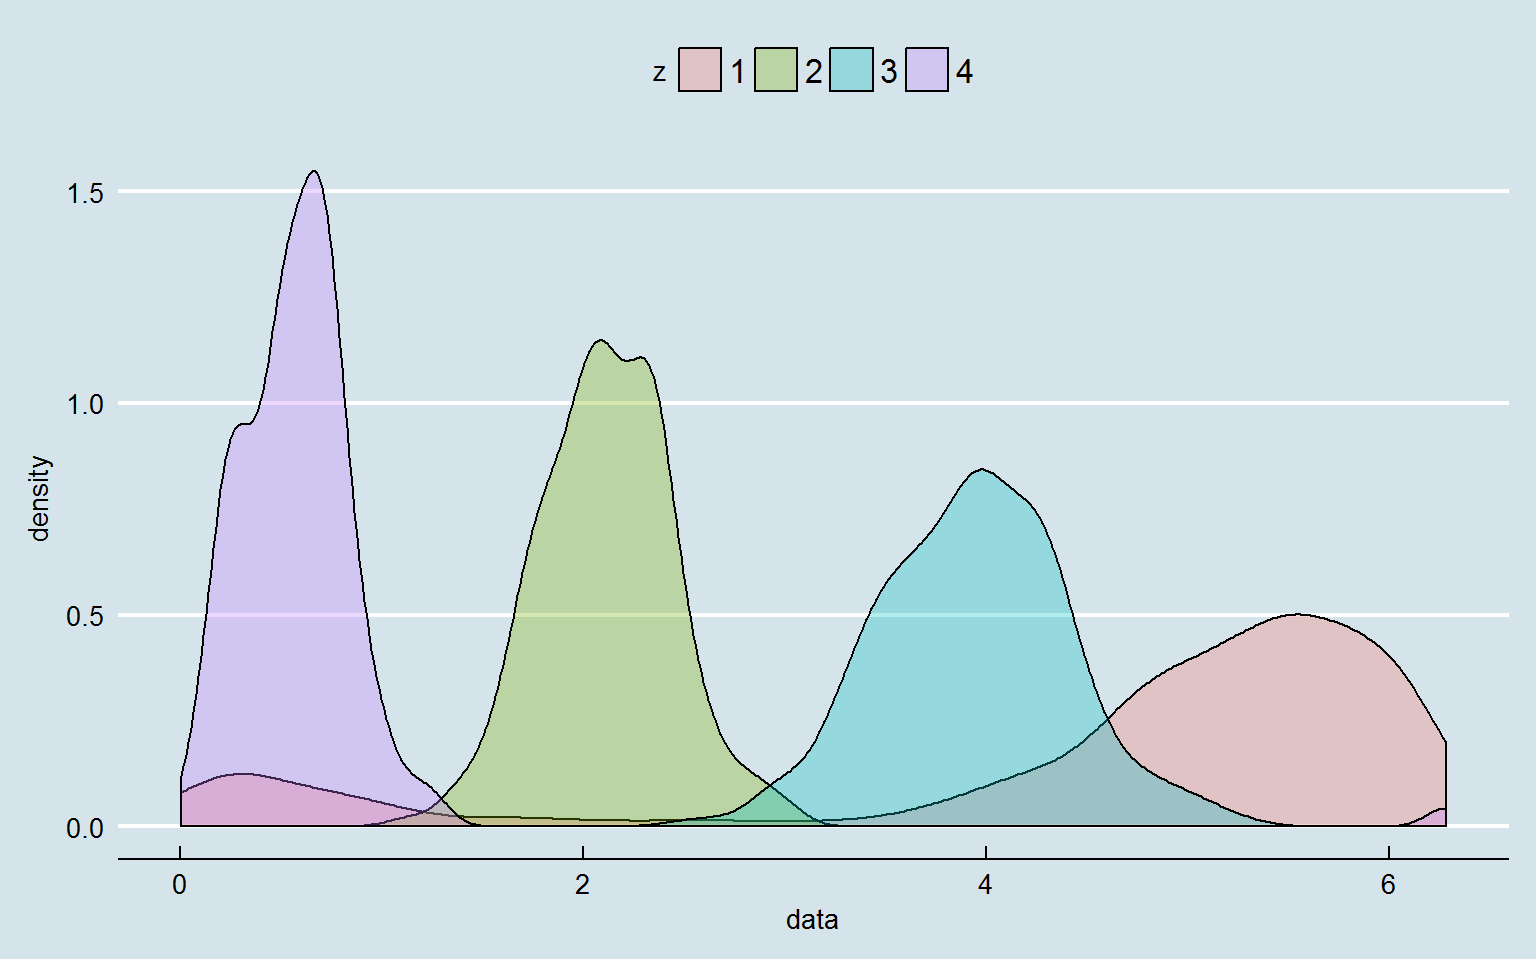
\includegraphics[clip,height= 35mm]{data/mix_test_data.png}
\end{center}
\caption{混合データ(クラスター数:4)}

\label{mixdata}
\end{figure}

\subsection{解析結果}

Mixture von Mises 分布では元のデータと同じく4つの元となる分布を推定したが, Mixture Projected Normal 分布においては3つの元となる分布により以下の結果が得られた.

\begin{figure}[tbp]
 \begin{tabular}{c}
\hspace{0.5cm}
 \begin{minipage}{0.5\hsize}
  \begin{center}
   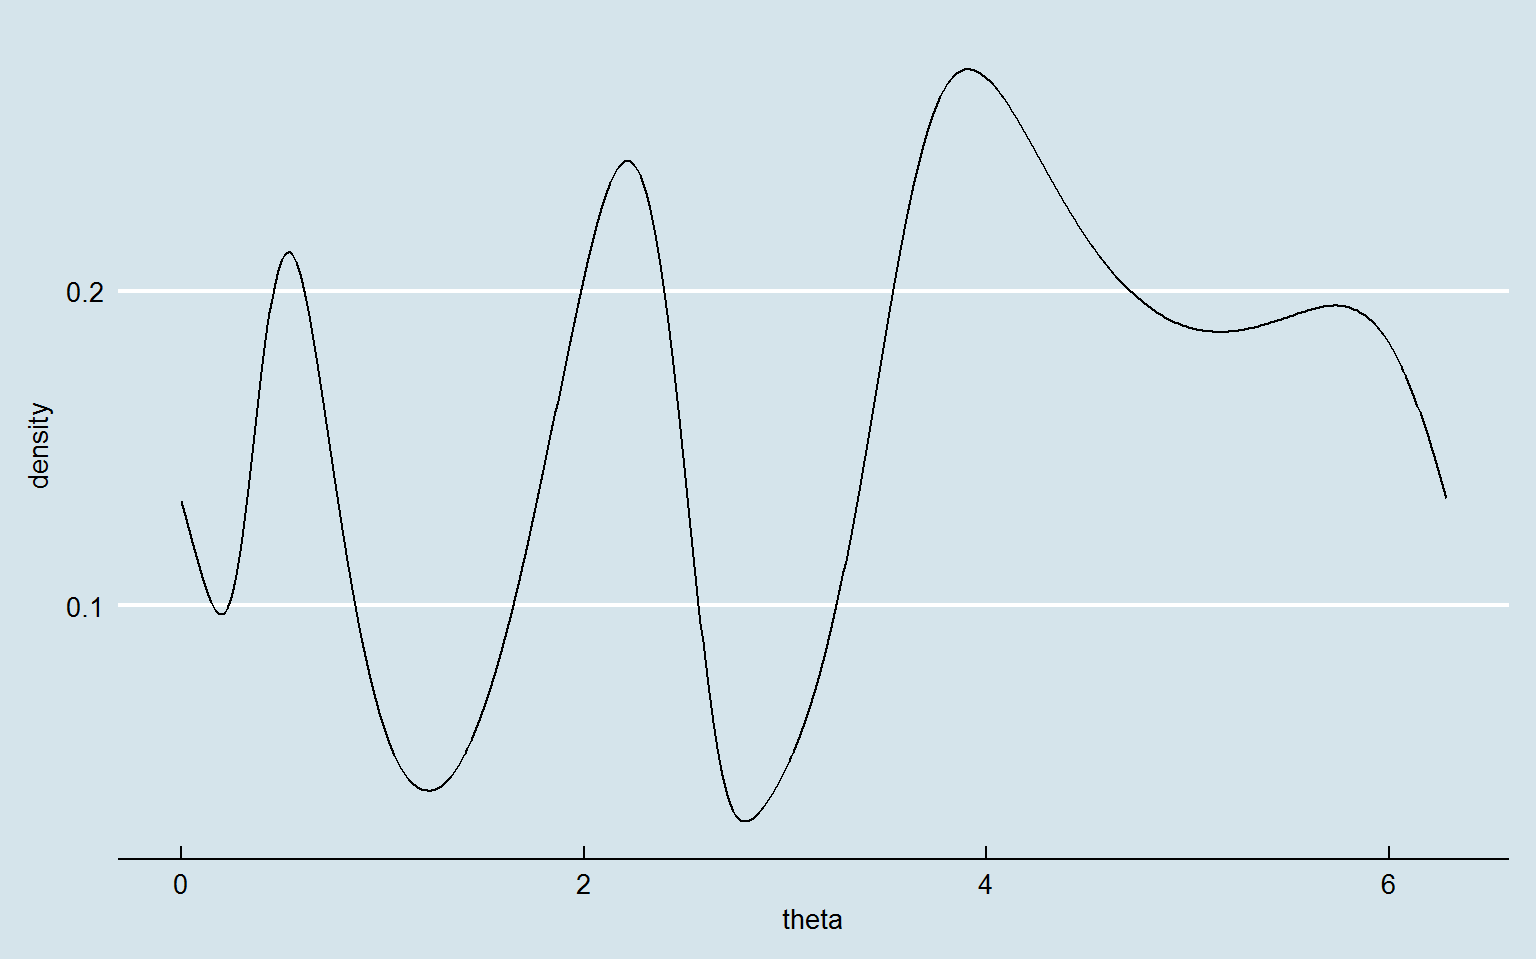
\includegraphics[clip,height= 35mm]{data/mix_pn.png}
  \end{center}
  %\caption{Mixture Projected Normal 分布により推定した混合分布}
  \label{pnmix}
 \end{minipage}
\hspace{-1.0cm}
 \begin{minipage}{0.5\hsize}
  \begin{center}
   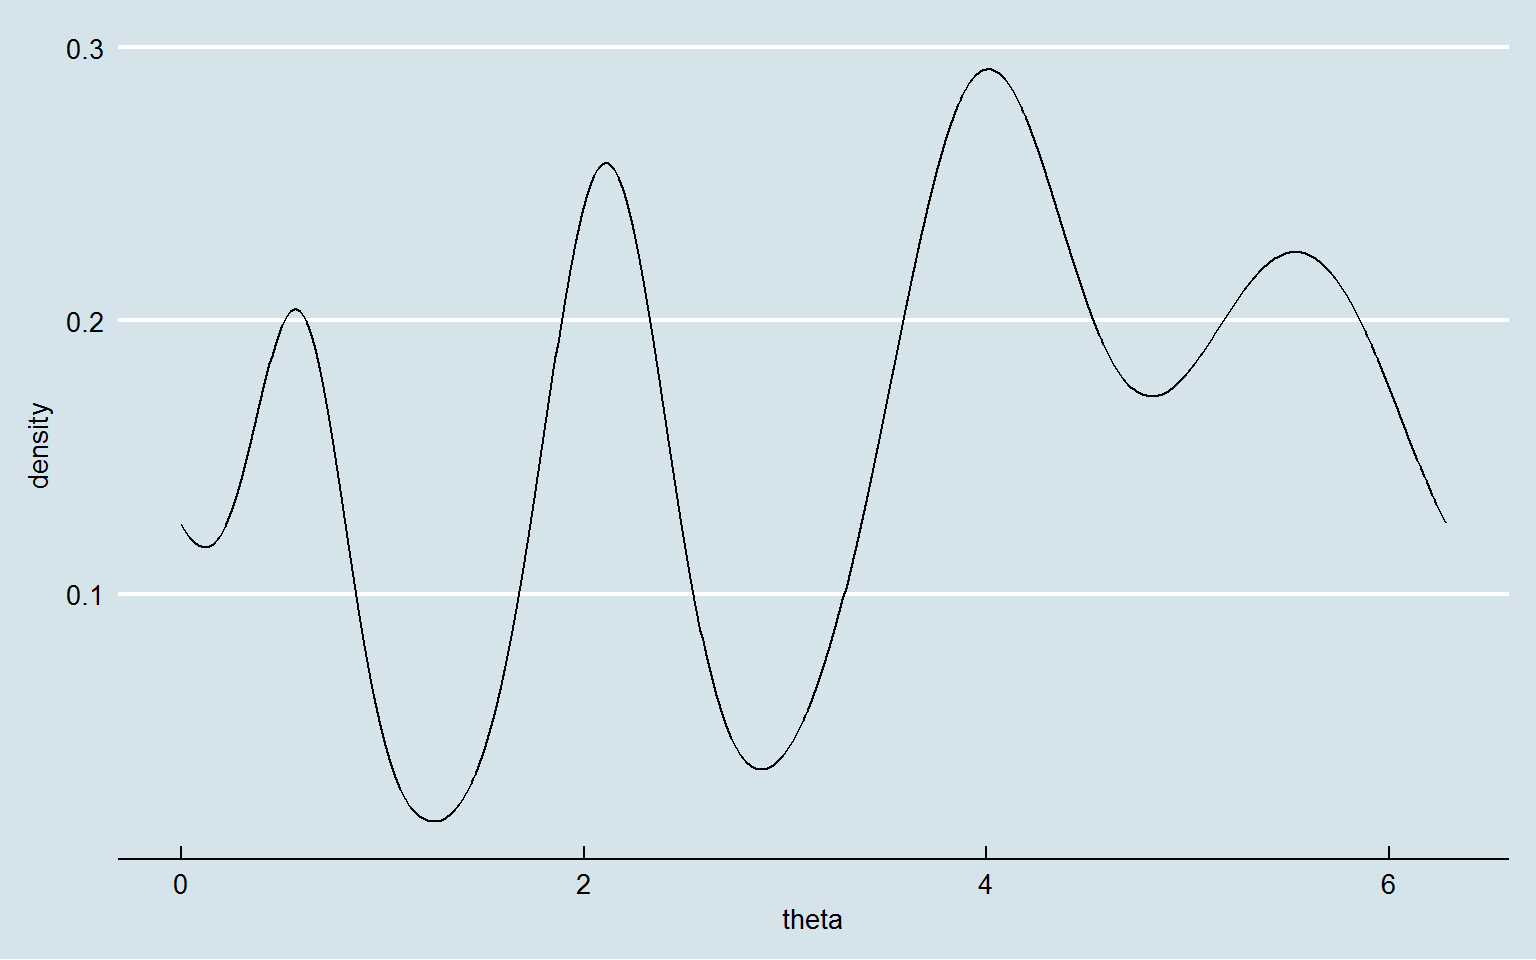
\includegraphics[clip,height= 35mm]{data/mix_von.png}
  \end{center}
 % \caption{Mixture von Mises分布により推定した混合分布}
  \label{vonmix}
 \end{minipage}
  \end{tabular}
\caption{Mixture Projected Normal 分布により推定した混合分布(左), Mixture von Mises分布により推定した混合分布(右)}
\end{figure}


得られた混合分布から, 混合データの分類を行う. 混合分布を構成する, 分布の中で出現確率が最も高いものをそのデータの予測クラスタとする.
横軸を真のクラスタ, 縦軸を予測クラスタとして集計表を示す. 

\begin{table}[tbp]
\caption{PN 分布によるクラスター推定(左), VM 分布によるクラスター推定(右)}
\begin{tabular}{c}
% 1
\hspace{1.5cm}
\begin{minipage}{0.5\hsize}
\begin{center}
%\caption{PN 分布によるクラスター推定}
\begin{tabular}{|c|c|c|c|c|}
\hline
 &  & \multicolumn{3}{|c|}{Predict} \\ \hline
 &  & 1 & 2 & 3 \\ \hline 
 &1 & 38 & 10 & 352 \\ \cline{2-5}
True
 & 2 & 1 & 192 & 7 \\ \cline{2-5}
 & 3 & 0 & 2  & 298 \\ \cline{2-5}
 & 4 & 93 & 0 & 7 \\ 
\hline
 \end{tabular}
 \end{center}
\end{minipage}

% 2
\hspace{-2.5cm}
\begin{minipage}{0.5\hsize}
\begin{center}
%\caption{VM 分布によるクラスター推定}
\begin{tabular}{|c|c|c|c|c|c|}
\hline
 &  & \multicolumn{4}{|c|}{Predict} \\ \hline
 &  & 1 & 2 & 3 & 4 \\ \hline 
 & 1 & 333 & 10 & 39 & 18 \\ \cline{2-6}
True
 & 2 & 7 & 192 & 1 & 0 \\ \cline{2-6}
 & 3 & 298 & 2  & 0 & 0 \\ \cline{2-6}
 & 4 & 0 & 1 & 94 & 5 \\ 
\hline
\end{tabular}
\end{center}
\end{minipage}

\end{tabular}
\end{table}
\fi

%%%%%%%%%%%%%%%%%%%%%%%%%%%%%%%%%%%%%%%%%%%%%%%%%%%%%%%%%%%%%%%%%%%
%%%%%%%%%%%%%%%%%%%%%%%  sectio4 数値実験 %%%%%%%%%%%%%%%%%%%%%%%%
\section{データ解析}

本章では, 実際のデータに対して混合射影正規分布によるクラスタリングを適用する. クラスターごとの特徴量を確認することで, 混合射影正規分布によるクラスタリングの妥当性を検証する.

\subsection{解析データ}

本研究では, \citet{MovieLens}による公開データセットMovieLensの一部分を用いた. MovieLensデータセットは映画評価サイト''movielens.com''において1997年9月から1998年4月までの7ヶ月間の間に集められた943人のユーザ, 1682個の映画についての10万個の評価値, 簡単なユーザ情報, コンテンツ情報から構成されている. 評価値において, $0$は見ていないことを表し, 評価については1から5までの5段階評価で数字が大きいほど高い評価である. 各ユーザは最低20個の映画に対する評価値を持っている. コンテンツ情報, ユーザ情報について表\ref{MovieLens1}にまとめる. また表\ref{MovieLens2}にMovieLensデータセットの一部を示す.

\begin{table}[bp]
\begin{center}
\caption{コンテンツ情報およびユーザ情報}   %キャプション
\label{MovieLens1}   %ラベル
\begin{tabular}{c l}
\hline
ジャンル & unknown, Action, Adventure, Animation, Children's, Comedy, \\
                 & Crime, Documentary, Drama, Fantasy, Film-Noir, Horror, Musical, \\
                 & Mystery, Romance, Sci-Fi, Thriller, War, Western \\
職業          & administrator, artist, doctor, educator, engineer, entertainment, executive, \\
                & healthcare, homemaker, lawyer, librarian, marketing, none, other, \\
                & programmer, retired, salesman, scientist, student, technician, writer \\
年齢 & 7歳 $\sim$ 73歳 \\
性別 & male, female\\ 
\hline
\end{tabular}
\end{center}
\end{table}

\begin{table}[tbp]
\begin{center}
\caption{MovieLens データセット例}   %キャプション
\label{MovieLens2}   %ラベル
\begin{tabular}{c c c c c c}
\hline
user-No	&	age	&	gender	&	occupation	&	item-No	& rating \\ \hline \hline
1	&	24	&	M	&	technician	&  1  & 5 \\	\hline
159	&    23	&     F	&      student	      &  274 & 3 \\	\hline
535	&	45	&	F	&	educator	&	511	& 3 \\ \hline
655	&	50	&	F	&	healthcare	& 393 & 2 \\	\hline
943	&	22	&	M	&	student	&	1330 & 3 \\  \hline
\end{tabular}
\end{center}
\end{table}

MovieLensのデータセットを用いて, 映画に対する評価値に基づいて, ユーザをクラスタリングする. MovieLensデータセットをユーザー($943$人)$\times$コンテンツ($1682$個)の行列データに変換する. この行列データは評価値の$94\%$が$0$であるスパースな行列として表すことができる. 映画の評価値において$0$から$6$の出現回数を表\ref{MovieLens3}に示す.

\begin{table}[tbp]
\begin{center}
\caption{映画に対する各評価値の出現回数}   %キャプション
\label{MovieLens3}   %ラベル
\begin{tabular}{c c c c c c}
\hline
0 & 1 & 2 & 3 & 4 & 5 \\ \hline 
1506126 & 4719 & 9178 & 21963 & 27396 & 16744 \\ \hline
\end{tabular}
\end{center}
\end{table}

\subsection{評価指標}

情報量基準(WAIC)を用いて, 混合分布のコンポーネントの選択を行う. AICやBICなどの情報量基準には, 事後分布が正規分布で近似されている必要があるなど, 様々な制約が存在するが, WAICは真の分布, 確率モデル, 事前分布がどのような場合でも用いることができる. WAICは式$(\ref{WAIC1})$で求められる.

\begin{eqnarray}
\label{WAIC1}
\mbox{WAIC} = T + \frac{V}{n}, 
\end{eqnarray}

\noindent
ここで, $T = - \frac{1}{n} \Sigma^n_{i=1} \log E_{\bm \eta}[p(\bm \theta_i| \bm \eta)], 
V = \Sigma^n_{i=1} \{ E_{\bm \eta}[(\log p(\bm \theta_i| \bm \eta))^2] - E_{\bm \eta}[\log p(\bm \theta_i| \bm \eta)]^2 \}$であり, $n$は$\bm \theta$のデータ数である. また$E_{\bm \eta}[\cdot]$は$\bm \eta$の事後分布の下で評価した期待値である.  

\subsection{クラスター分析}

t-SNEを用いて高次元データを$3$次元に圧縮する. 得られた$3$次元データをノルムで割ることで正規化し, 極座標変換することで角度データ$\bm \theta = (\theta_1, \theta_2)^T$を取得する. t-SNEにより得られた異なる$10$個の$3$次元データに対し, コンポーネントを$1$から$4$まで変化させた場合のWAICを表$\ref{WAIC2}$に示す. 


\begin{table}[tbp]
\caption{WAICによるコンポーネントの選択結果}
\label{WAIC2}
\begin{center}
\scalebox{0.75}{
\begin{tabular}{l | c c c c c c c c c c}
\hline
 & 1 & 2 & 3 & 4 & 5 & 6 & 7 & 8 & 9 & 10 \\ \hline \hline 
$m=1$ & -1014.1 & -1237.0 & -1350.6 & -1009.5 & -1308.8 & -1227.8 & -1152.4 & -902.5 & -1322.6 & -1140.2 \\ 
$m=2$ & -1610.9 & -1675.0 & -1760.4 & -1552.8 & -1633.1 & -1529.6 & -1507.1 & -1366.1 & -1645.2 & -1693.3 \\ 
$m=3$ & -1846.8 & -1744.7 & -1728.9 & -1804.9 & -1741.0 & -1654.3 & -1705.2 & -1633.8 & -1789.3 & \textbf{-1872.1} \\ 
$m=4$ & \textbf{-1893.6} & \textbf{-1969.8} & \textbf{-1901.6} & \textbf{-1837.5} & \textbf{-1787.5} & \textbf{-1687.8} &\textbf{-1749.5} & \textbf{-1686.7} & \textbf{-1844.5} & -1802.6 \\ 
\hline
\end{tabular}
}
\end{center}
\end{table}


\noindent
$9$個のデータにおいて, コンポーネントが$4$つのときWAICが最小になっていることがわかる. コンポーネントを$4$つと仮定して混合射影正規分布によるクラスタリングを行う. HMCによって推定された, $4$つのコンポーネントにおける混合射影正規分布のパラメータを式(\ref{parameter})に示す. なお, $\hat {\bm w}$は各コンポーネントの混合比率を表し, パラメータの添え字はコンポーネントの番号に対応している.

\begin{equation}
\label{parameter}
\begin{split}
&\hat {\bm w} = \begin{pmatrix} 0.26 \\ 0.51 \\ 0.20 \\ 0.03 \\ \end{pmatrix},\ 
\hat{\bm \mu}_1 = \begin{pmatrix} 0.44 \\ 2.85 \\ -1.67 \\ \end{pmatrix},\ 
\hat \Sigma_1 = \begin{pmatrix}  2.40 & 1.52 &  0.06 \\ 1.52 & 2.20 & -0.25 \\ 0.06 & -0.25 &1.00 \\ \end{pmatrix},\\ 
&\hat{\bm \mu}_2 = \begin{pmatrix} 0.14 \\ -0.50 \\ 1.09 \\ \end{pmatrix},\ 
\hat \Sigma_2 = \begin{pmatrix}   0.28  & 0.14 &  0.20 \\ 0.14 & 0.61 & 0.06 \\  0.20 & 0.06 &1.00 \\ \end{pmatrix},\ 
\hat{\bm \mu}_3 = \begin{pmatrix} -2.08  \\ -1.96 \\ -8.11 \\ \end{pmatrix},\\ 
&\hat \Sigma_3 = \begin{pmatrix}  1.86  & -0.18 &  -0.10 \\-0.18 & 3.89 & 1.60 \\  -0.10 & 1.60 & 1.00 \\ \end{pmatrix},\ 
\hat{\bm \mu}_4 = \begin{pmatrix} -12.29   \\ -2.48 \\ -4.84 \\ \end{pmatrix},\ 
\hat \Sigma_4 = \begin{pmatrix} 15.19 & 4.01 &  0.12 \\ 4.01 & 1.88 & 0.08 \\ 0.12 & 0.08 &1.00 \\ \end{pmatrix}.
\end{split}
\end{equation}

得られたパラメータベクトル$\bm \eta$と$3$次元データを用いて, 混合分布によるクラスタリングを行う. 球面上におけるクラスタリング結果を図\ref{clusterplot3d}に示す. ここで, 中心部からの各矢線は各コンポーネントの平均方向を表す. また球面上の角度$\bm \theta = (\theta_1, \theta_2)^T$における, クラスタリング結果を図\ref{clusterplot2d}に示す.

\newpage %この図は1ページにする
\begin{figure}[tbp]
\begin{center}
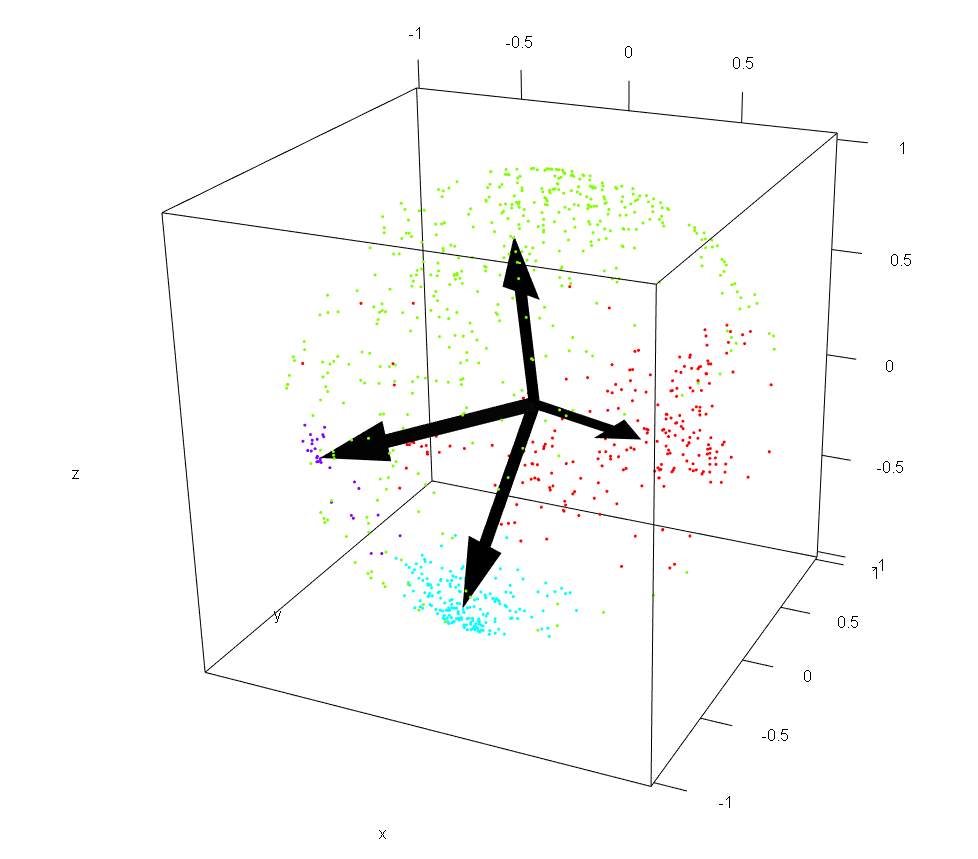
\includegraphics[clip,height= 140mm]{data/cluster_3d.png}
\end{center}
\caption{混合分布による, 球面上におけるクラスタリング結果}
\label{clusterplot3d}
\end{figure}

\newpage %この図は1ページにする
\begin{figure}[tbp]
\begin{center}
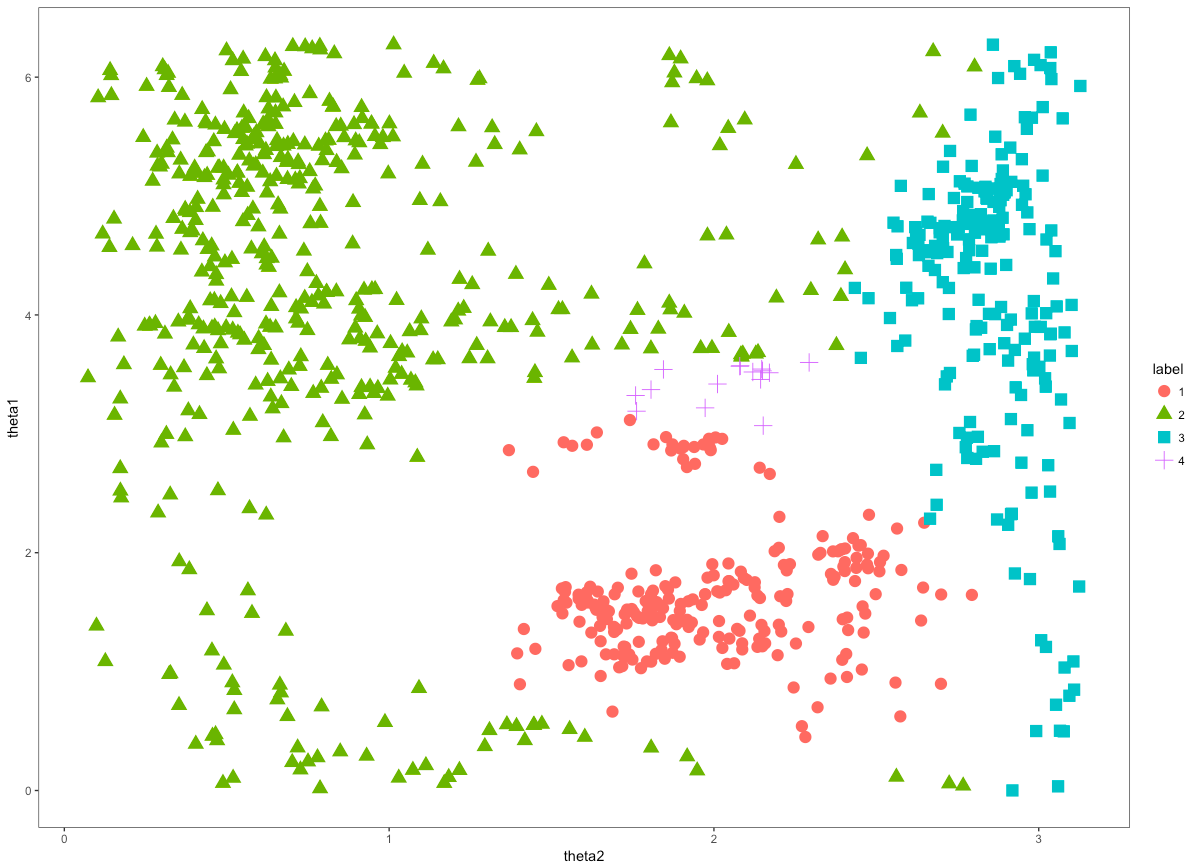
\includegraphics[clip,height= 110mm]{data/cluster_4.png}
\end{center}
\caption{混合分布による, 球面上の角度$\bm \theta = (\theta_1, \theta_2)^T$におけるクラスタリング結果}
\label{clusterplot2d}
\end{figure}

\newpage
\clearpage
各ユーザの評価値と各映画のジャンル($19$種類)を用いて, ユーザごとに各ジャンルへの総評価値を算出する. 各映画には複数のジャンルが対応している. ユーザごとに全ての映画に対して, 

\begin{equation*}
\mbox{(任意の映画に対する評価値)} \times \mbox{(任意の映画のジャンル)},
\end{equation*}

\noindent
を算出し, 総和をとることで, ユーザごとに各ジャンルへの総評価値を求めた. これらの計算は, ユーザー($943$人)$\times$コンテンツ($1682$個)の行列とコンテンツ($1682$個)$\times$ジャンル($19$個)の行列の演算に相当しており, 省略形を式(\ref{user_genre_matrix})に示す. 

\begin{equation}
\label{user_genre_matrix}
\begin{pmatrix} 
5 & 3 & 4 & 3 & \ldots & 0 \\
4 & 0 & 0 & 0 & \ldots & 0 \\
\vdots & \vdots & \vdots & \vdots & \ddots & \vdots \\
0 & 5 & 0 & 0 & \ldots & 0 \\
\end{pmatrix} 
\times
\begin{pmatrix} 
0 & 0 & \ldots & 0 \\
0 & 1 & \ldots & 0 \\
0 & 0 & \ldots & 0 \\
0 & 1 & \ldots & 0 \\
\vdots & \vdots & \ddots & \vdots \\
0 & 0 & \ldots & 0 \\
\end{pmatrix}
=
\begin{pmatrix} 
0 & 95 & \ldots & 4 \\
0 & 17 & \ldots & 0 \\
0 & 17 & \ldots & 0 \\
\vdots & \vdots & \ddots & \vdots \\
0 & 227 & \ldots & 23 \\
\end{pmatrix},
\end{equation}

\noindent
ここで, 得られたユーザごとジャンルへの評価値から, コンポーネントごとのジャンルへの評価値を求めることを考える. 図\ref{genre_count}に示したように, 各ジャンルは均等に出現していないので, 各ジャンルの影響を基準化する必要がある. 式(\ref{user_genre_matrix})で得られた行列を各列ごとに標準偏差で割ることで, 正規化を行う. 

\begin{figure}[H]
\begin{center}
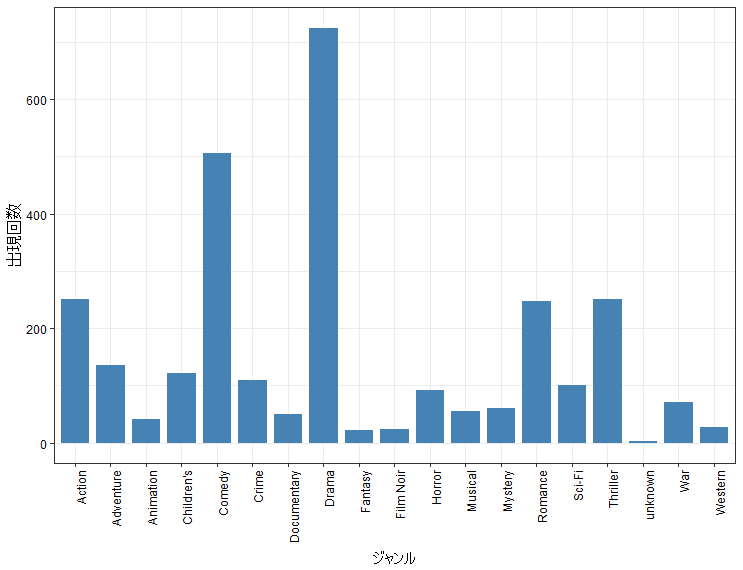
\includegraphics[clip,height= 100mm]{data/genre_count.png}
\end{center}
\caption{コンテンツの各ジャンルの出現回数}
\label{genre_count}
\end{figure}

\begin{figure}[H]
\begin{center}
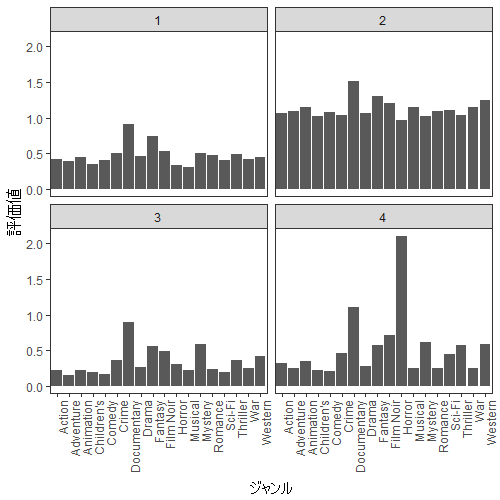
\includegraphics[clip,height= 100mm]{data/cluster_plot.png}
\end{center}
\caption{クラスターごとのジャンルへの評価値}
\label{clustergenre}
\end{figure}

%\newpage
正規化したユーザごとジャンルへの評価値から, コンポーネントごとのジャンルへの評価値を求めた. 結果を図\ref{clustergenre}に示す. クラスター$2$は幅広いジャンルの映画に対して, 高評価を与えているユーザが所属し, クラスター$1,3,4$ではジャンルへの評価値に差が現れた. 
MovieLensのデータセットには映画のジャンルに加えて, ユーザの簡単な情報も記載されている. 各コンポーネントにおいて, ユーザの評価値の平均値, ユーザの平均年齢, 所属するユーザ数を表\ref{component_stat}にまとめる. また, 各コンポーネントにおける平均評価値, 所属するユーザの年齢と職業の出現回数を図\ref{rating_average}, 図\ref{job_count}, 図\ref{age_count}に示す. 結果から分かるように, 各コンポーネントの特徴は現れなった. 表\ref{component_stat}より, 混合分布によるクラスタリングでは所属ユーザにばらつきが生まれてしまうことが分かる. ユーザの評価値に基づいて, クラスリング分析を行っているので, ユーザの評価値の特徴とユーザの属性の特徴が対応している必要がある. しかし, ユーザの映画に対する評価値において$0$の値が非常に多く, $0$のデータを特徴として扱うと, 各ユーザの特性がわかりにくくなる可能性がある. 実際には$0$のデータはまだ見ていないことを表しており, 数値的な意味が存在しないので, $0$のデータを取り除いて考える必要がある.

\begin{table}[H]
\begin{center}
\caption{各コンポーネントにおけるユーザ情報の平均値と所属ユーザ数}   %キャプション
\label{component_stat}   %ラベル
\begin{tabular}{c | c c c c}
\hline
&1 & 2 & 3 & 4 \\ \hline \hline
平均評価値 &3.576 & 3.653 & 3.453 & 3.606 \\ \hline
平均年齢 & 34.5 &  33.5 & 35.4 & 28.4 \\ \hline
所属ユーザ数 & 244 & 468 & 202 & 29 \\ \hline
\end{tabular}
\end{center}
\end{table}

\begin{figure}[tbp]
\begin{center}
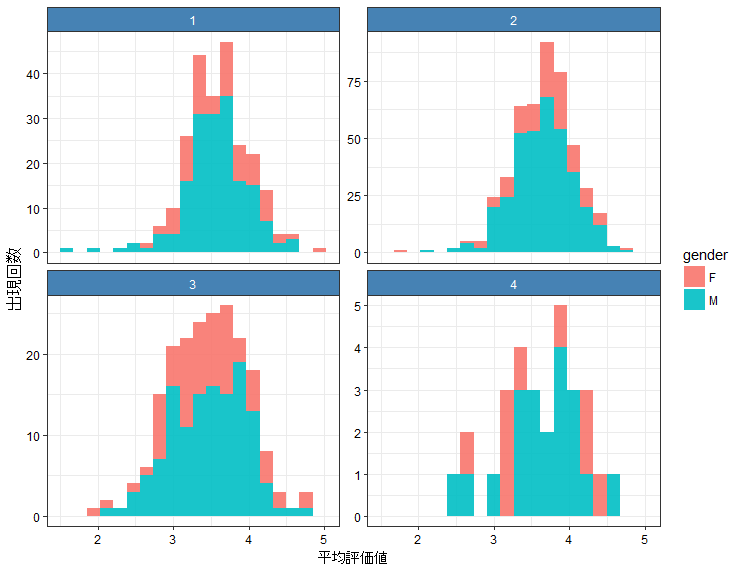
\includegraphics[clip,height= 130mm]{data/rating_average.png}
\end{center}
\caption{各コンポーネントの平均評価値}
\label{rating_average}
\end{figure}

\begin{figure}[tbp]
\begin{center}
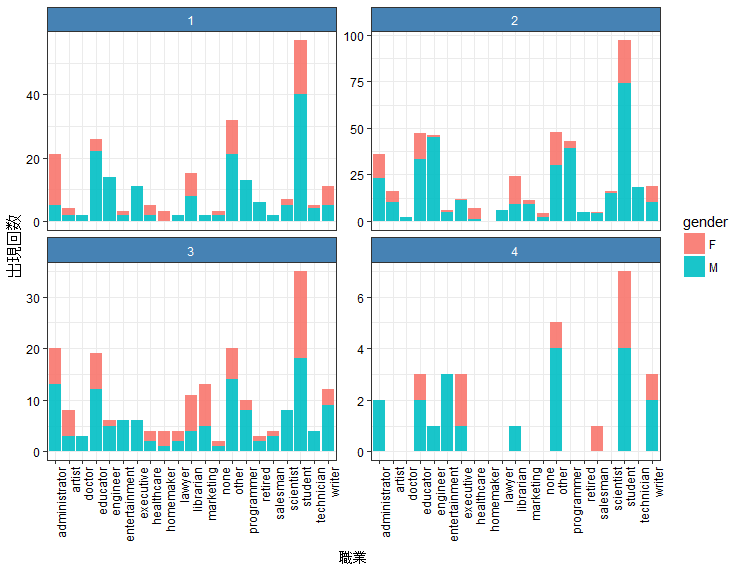
\includegraphics[clip,height= 130mm]{data/job_count.png}
\end{center}
\caption{各コンポーネントに所属するユーザの職業の出現回数}
\label{job_count}
\end{figure}

\begin{figure}[tbp]
\begin{center}
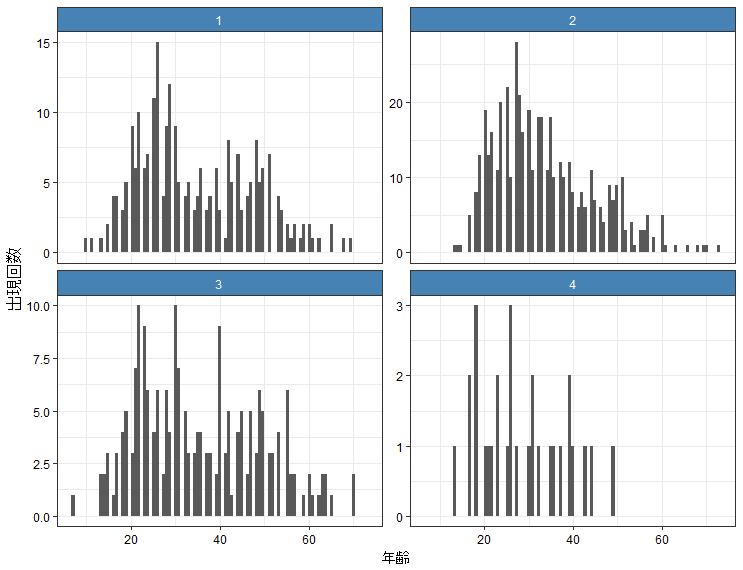
\includegraphics[clip,height= 130mm]{data/age_count.png}
\end{center}
\caption{各コンポーネントに所属するユーザの年齢の出現回数}
\label{age_count}
\end{figure}

%%%%%%%%%%%%%%%%%%%%%%%  section5 まとめ %%%%%%%%%%%%%%%%%%%%%%%%%%%%%
\newpage
\section{まとめと今後の課題}

本研究では計算量の問題で高次元データをあらかじめ$3$次元に圧縮し, クラスタリングを試みたが, クラスターごとの特徴を明確に抽出することができなかった. 一般化射影正規分布では任意次元の超球面において分布を生成することができるので, 計算量の問題を解決し, 次元を圧縮することなく超球面上でのクラスタリングに取り組みたい. 本研究では数値データを球面上に配置し, クラスタリングを行ったのが, 超球面上でのクラスタリングは主にテキストマイニングや画像データに用いられているので, それらのデータに対するパラメトリックなクラスタリングを行い, 従来手法との比較を行いたい. 

%%%%%%%%%%%%%%%%%%%%%%%  謝辞 %%%%%%%%%%%%%%%%%%%%%%%%%%%%%
\section{謝辞}

本研究を行うにあたり, ご指導を頂いた塩濱教授に感謝しています. この一年間で, 卒業研究だけでなく, 興味を持った多くのことに対して取り組むことができました. またお忙しい中, 学部生の質問に対応して頂いた院生の皆様にも感謝しています. 同期の皆様のおかげで, 卒業研究や研究室行事を協力して乗り切ることができたと思っています. 特に黒木君は大学院に進む友人として, 共に切磋琢磨し, お互いを鼓舞することができたと思います. 最後になりますが, ここまで支えてくれた両親に感謝しています.

\newpage
\addcontentsline{toc}{section}{参考文献} %目次に参考文献を入れる

%参考文献を引用する際に必要なコマンド
%\bibliographystyle{jplain}
\bibliography{bunken}

%\newpage
%\section{付録}

\end{document}